\documentclass{article}
\usepackage{graphicx} % Required for inserting images
\usepackage{geometry}
\usepackage[font=small,labelfont=bf]{caption}
\usepackage{subcaption}
\usepackage{float}
%\usepackage{titlesec}
\usepackage[hidelinks, colorlinks=true, allcolors=blue]{hyperref}
\usepackage[french]{babel}
\addto\captionsfrench{\def\tablename{Tableau}}
\usepackage{breqn} % for dmath
\usepackage{siunitx}
\usepackage[T1]{fontenc}
\usepackage{listings}
\usepackage{cleveref}

\geometry{a4paper, margin=1.9cm}

\edef\restoreparindent{\parindent=\the\parindent\relax}
\usepackage{parskip}

\title{TP 3 : Interférences et Diffraction}
\author{Pauline Toutain, Hervé Schmit-Veiler}
\date{Avril 2024}


\begin{document}

\maketitle

\section{Diffraction à l'infini par une fente de largeur $b$}
\label{sec:diffraction}

La première expérience consiste à observer la figure de diffraction formée lorsqu'on 
éclaire une fente fine de largeur $b$ avec une faisceau laser collimaté et monochromatique.

Le montage expérimental consiste d'un laser, d'une fente et d'un écran placé le long d'un banc optique.
L'orientation du laser et la position de la fente on été ajustée afin que le faisceau laser soit en incidence normale avec 
le centre de la fente. Pour assurer la fiabilité de nos measures, 
il à aussi fallu orienter l'écran parallel à la fente, afin que la figure de diffraction puisse être lue sans 
distortion.

La distance fente-écran $D$ est particulièrement importante dans cette expérience. 
Lorsque l'écran est trop près de la fente ($D \approx 10 \text{ cm}$), 
le nombre de Fresnel $N$ n'est plus très petit devant l'unité. 

$$N = \frac{b^2}{\lambda D} \sim \frac{(50\times10^{-6})^2}{500\times10^{-9} \cdot 10\times10^{-2}} = 0.05$$

Donc, pour se placer dans le régime de Fraunhofer 
il faut s'assurer que l'écran soit placé suffisamment loin derrière la fente.

Avec l'écran au bout du banc (donc en régime de Fraunhofer), on observe en variant 
la largeur de la fente que la figure de diffraction se comprime 
(les maxima se rapprochent) lorsqu'on élargit la fente, et vice versa.
  
\begin{figure}[H]
    \centering
    \begin{subfigure}[b]{0.3\textwidth}
        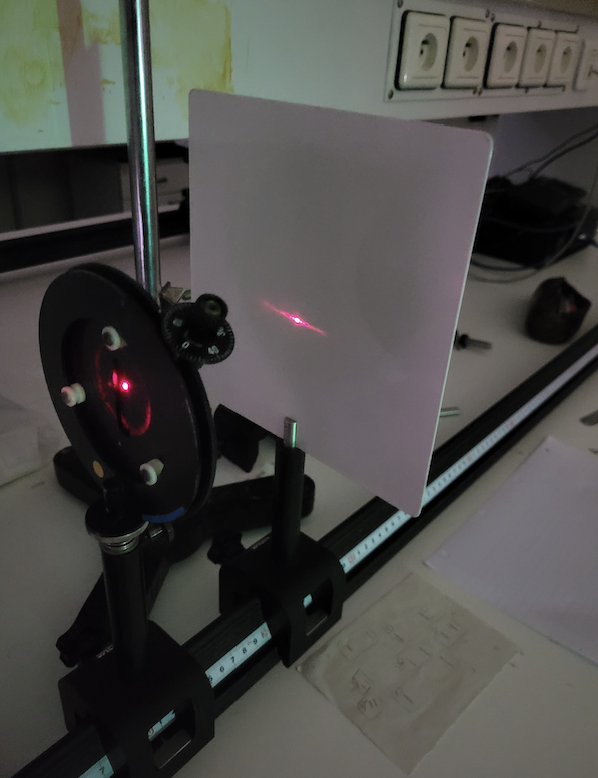
\includegraphics[width=\textwidth]{figs/fraunhofer_1.png}
        \caption{}\label{fig:fraunhofer_1}
    \end{subfigure}
    \begin{subfigure}[b]{0.3\textwidth}
        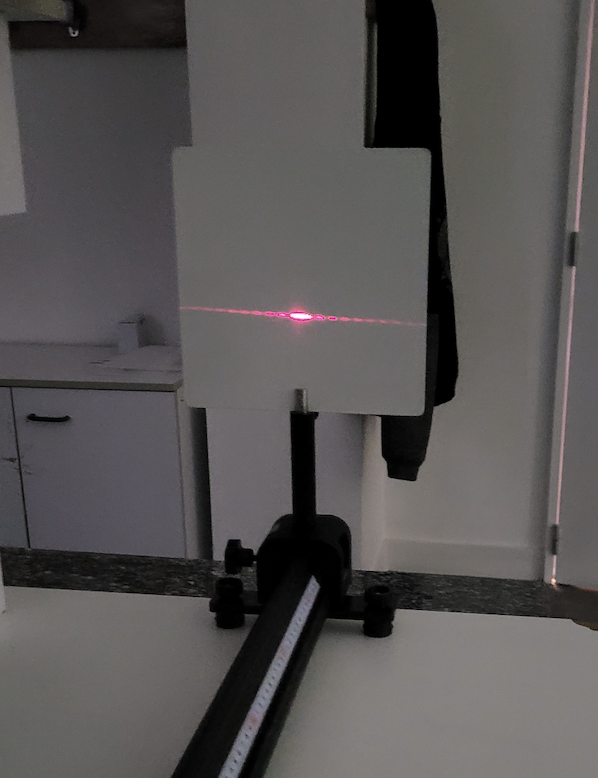
\includegraphics[width=\textwidth]{figs/fraunhofer_2.png}
        \caption{}\label{fig:fraunhofer_2}
    \end{subfigure}
    \caption{Figure de diffraction en dehors du régime de Fraunhofer à $D \approx 10 \textrm{ cm}$ \textbf{(a)}. 
    Figure de diffraction dans le régime de Fraunhofer à $D \approx 2 \textrm{ m} $ \textbf{(b)}.}
    \label{fig:diff_1}
\end{figure}

\subsection{Mesurer la largeur du maxima central}

En gardant le même montage que pour nos observations préliminaires, nous avons 
mesuré la largeur du maxima central $\Delta y$ en fonction de la largeur de la 
fente $b$ en marquant les positions des deux minima symétriques d'ordre 1 sur une 
feuille placé sur l'écran – mesures qui ont été répétées pour 7 fentes différentes, dont une avec une largeur inconnue que l'on va chercher à trouver.

Nous avons mesuré la distance entre les deux minima avec une règle pour obtenir $\Delta y$. 

Toutes ces mesures ont été prises avec un laser rouge $\lambda_r = 650 \textrm{ nm}$, 
à une distance $D = 170 \pm 0.05 \textrm{ cm}$ de la fente. 


\begin{table}[H]
\begin{center}
    \begin{tabular}{|c|c|}
    \hline
    $b$ (µm) & $\Delta y$ ($\pm 0.1 \textrm{ cm}$) \\
    \hline
    $400$ & $0.55$ \\
    $280$ & $0.83$ \\
    $120$ & $1.92$ \\
    $100$ & $2.29$ \\
    $50$ & $4.87$ \\
    $40$ & $6.30$ \\
    ? & $3.56$ \\
    \hline
\end{tabular}
\end{center}
\caption{Valeurs de $a$ et $b$ obtenus à partir des relations théoriques}
\end{table}

Dans le régime de Fraunhofer, la larguer du maxima central de la figure de diffraction $\Delta y$ est donné par la formule suivante :

\begin{equation}
    \Delta y = 2 \frac{\lambda D}{b}
\end{equation}

Donc selon cette relation, $2\lambda D = 2.21 \times 10^{-6} \textrm{ m}^2$. Sachant aussi que $\Delta y$ varie de manière monotone en fonction de $b$, on peut déjà s'attendre
à trouver une largeur pour la fente mystère $b_{\textrm{mystère}}$ entre $50 \textrm{ µm}$ et $100 \textrm{ µm}$.


\begin{figure}[H]
    \centering
    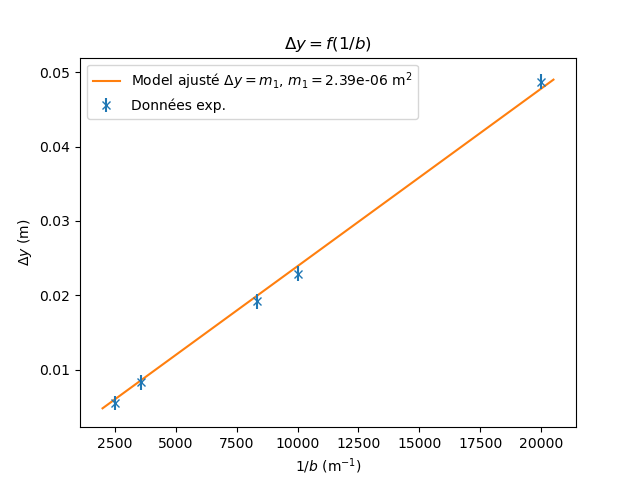
\includegraphics[width=0.6\linewidth]{figs/diff_1.png}
    \caption{Tracé des données expérimentales $\Delta y = f(1/b)$ (croix bleus), avec ajustement linéaire.}
    \label{fig:diff_1}
\end{figure}

Un ajustement linéaire a été obtenu avec la librairie python {\color{blue}scipy.optimize.curve_fit}, le coefficient directeur 
ainsi trouvé de $m_1 = (2.39 \pm 0.04)\times 10^{-6} \textrm{ m}^2$ ne contient pas la 
prédiction théorique dans ses incertitudes. Or, le nombre de mesures étant vraiment assez faible, 
cet écart de $\sim 8\%$ n'est pas aberrant. L’incertitude de $m_1$, correspondant à un écart type, provient aussi de la fonction {\color{blue}curve_fit}.

Sachant que pour la fente mystère $\Delta y = 3.56 \pm 0.1 \textrm{ cm}$, on obtient la largeur suivante qui se trouve bien dans l'intervalle suggérée précédement :

$$ b_{\textrm{mystère}} = \frac{m_1}{\Delta y} = 67.1 \pm 2 \textrm{ µm}$$

\section{Interférences à deux ondes - dispositif de Young}

Dans cette seconde expérience, nous avons experimenté avec les interérences crées en 
pointant un faisceau laser sur une bifente de largeur $b$ et de distance $a$ entre les deux fentes.
La largeur des fentes étant suffisament proche de l'ordre de grandeurs des longeurs d'ondes optiques, on observe une figure d'interférences 
modulée par une figure de diffraction. 
Nous avons étudié la figure d'interférences (en particulier l'interfrange $i$) crée en fonction des paramètres de la bifente.

Le montage expérimentale est similaire à celui utilisé dans section \ref{sec:diffraction}, le fente simple étant remplacée par un 
composant rotatif comportant trois bifentes de dimension différentes. Une fois de plus, l'orientation
et la position des composants ont été ajustées pour que le faisceau laser soit toujours en incidence normale, éclairant les
deux fentes de manière symétrique.

\subsection{Fentes de Young – partie 1}
Pour cette première partie, on tente de trouver $a$ et $b$ de manière experimentale. On fixe à présent la valeur fentes-écran à $D = 180 \pm 0.05 \textrm{ cm}$.
Se trouvant toujours dans le régime de Fraunhofer, on peut déduire $b$ en measurant $\Delta y$ de l'envelope de diffraction (même méthode qu'avant).
Les mesures d'interfranges sont obtenues en faisant la moyenne sur une dizaine de franges brillantes, ce qui nous permet d'avoir un mesure plus précise.

Lorsqu'on reste près de l'axe optique (angle $\theta$ de vue petit), on obtient la formule suivante pour l'interfrange :

\begin{equation}
    i = \lambda \frac{D}{a}
    \label{eq:interfrange}
\end{equation}


À l'aide de ces relations théoriques on obtient les valeurs et incertitudes de $a$ et $b$ pour chacune des trois 
bifentes.

%$\Delta a$ fait référence à l'incertitude de mesure de la variable $a$.
%$$\Delta a = \sqrt{\left(\frac{\lambda}{i}\Delta D\right)^2 + \left(\frac{\lambda D}{i^2} \Delta i \right)^2}$$
\begin{table}[H]
\begin{center}
    \begin{tabular}{|c|c|c|}
    \hline
    $i$ (mm) & $a$ (µm) & $b$ (µm) \\
    \hline
    $5.83 \pm 0.3$ & $201 \pm 6$ & $70.9 \pm 6$ \\
    $3.75 \pm 0.1$ & $312 \pm 9$ & $67.8 \pm 9$ \\
    $2.35 \pm 0.08$ & $499 \pm 10$ & $66.9 \pm 10$ \\
    \hline
\end{tabular}
\end{center}
\caption{Valeurs de $a$ et $b$ obtenus à partir des relations théoriques}
\end{table}

\subsection{Fentes de Young – partie 2}
Pour cette seconde partie, nous avons mesuré l'interfrange pour des distances $D$ differentes en utilisant la troisième bifente $a = 499\pm10 \textrm{ µm}$.
Après avoir tracé $i$ en fonction de $D$, on fait un ajustement linéaire avec coefficient directeur $m_2$.

\begin{figure}[H]
    \centering
    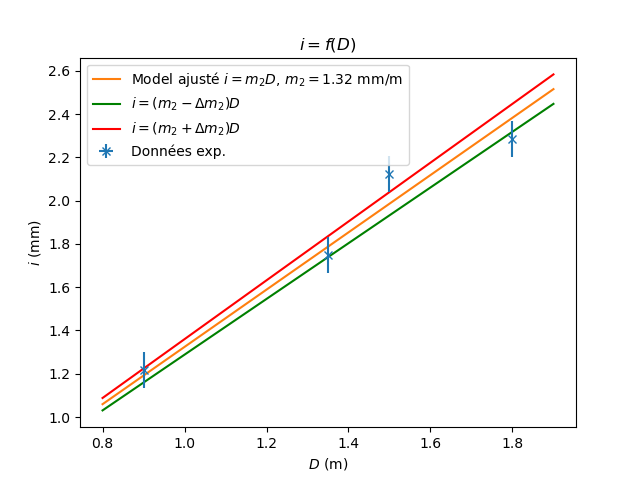
\includegraphics[width=0.6\linewidth]{figs/young_2_i=f(D).png}
    \caption{Tracé des données expérimentales $i=f(D)$ (croix bleues) avec ajustement linéaire (courbe orange). 
    On trace aussi les ajustements de pente maximale (courbe rouge) et de pente minimale (courbe verte) pour illustrer les valeurs de $m_2$ inclues dans les incertitudes.}
    \label{fig:diff_1}
\end{figure}

L'incertitude relative de $D$ étant très petite par rapport à celle de $i$ ($\frac{\Delta D}{D}<0.07\%$, indiscernable sur le tracé), 
on décide de la négliger dans le calcul de l'incertitude $\Delta m_2$. 
Cela nous permet de continuer d'utiliser la fonction {\color{blue}curve_fit}, 
qui ne prend en compte que l'incertitude de la variable dépendente.

$$i = \lambda \frac{D}{a} = m_2 D \qquad m_2 = \frac{\lambda}{a}$$

Connaissant déjà $a$ pour cette bifente, il nous est maintenant possible de vérifier la longeur d'onde de notre laser. 
Pour le laser rouge, on trouve $\lambda = 660 \pm 26 \textrm{ nm}$, valeur experimentale concordant
avec la longeur d'onde de $650 \textrm{ nm}$ donnée par le fabricant.

\subsection{Fentes de Young – partie 3}

En fixant $D = 170 \pm 0.05 \textrm{ cm}$, on mesure l'interfrange de la figure de diffraction avec un laser vert et un laser bleu avec 
la même bifente $a = 499\pm10 \textrm{ µm}$. Ayant déjà mesuré l'interfrange du laser rouge dans ces mêmes conditions, 
on en déduit la longeur d'onde des trois lasers à partir de la relation théorique \eqref{eq:interfrange} : 

\begin{table}[H]
    \begin{center}
        \begin{tabular}{|c|c|c|c|}
        \hline
        Laser & $i$ (mm) & $\lambda_{\textrm{exp}}$ (nm) & $\lambda_{\textrm{fabricant}} \textrm{ (nm)}$\\
        \hline
        Rouge & $2.28 \pm 0.08$ & $ 633 \pm 30$ & $650$ \\
        Vert & $1.95 \pm 0.05$ & $540 \pm 20$ & $535$ \\
        Bleu & $1.47 \pm 0.08$ & $409 \pm 30$ & $405$ \\
        \hline
    \end{tabular}
    \end{center}
    \caption{Valeurs de $i$ avec les longeurs d'ondes de chaque laser déduit experimentalement à partir de \eqref{eq:interfrange} pour $a = 499\pm10 \textrm{ µm}$ et $D = 170 \pm 0.05 \textrm{ cm}$. 
    Les longeurs d'ondes fournies par le fabricants sont aussi notées dans la colonne à droite.}
\end{table}

Nous obtenons des valeurs $\lambda$ qui sont en accord avec celles données par le fabriquant, ainsi qu'avec nos mesures précédentes (pour le laser rouge). 
On vérifie, avec un ajustement linéaire, qu'en effet les variations de l'interfrange en fonction de la longeur d'onde vérifient bien la relation théorique linéaire \eqref{eq:interfrange}.

\begin{figure}[H]
    \centering
    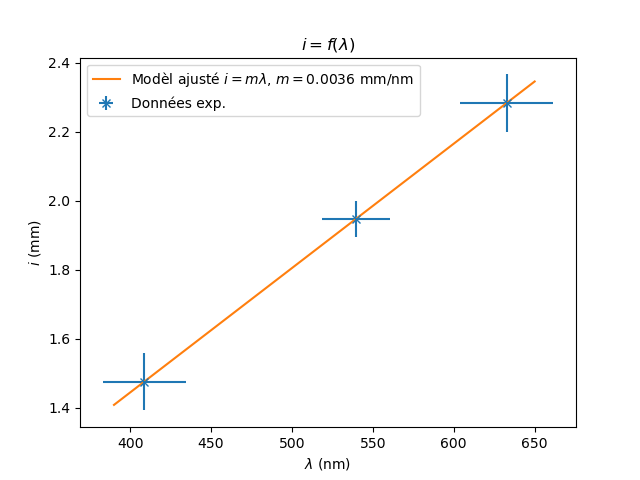
\includegraphics[width=0.6\linewidth]{figs/i=f(lambda).png}
    \caption{Tracé des données expérimentales $i=f(\lambda)$ (croix bleus) avec ajustement linéaire (courbe orange).}
    \label{fig:verif_lambda}
\end{figure}

\section{Interférences à N ondes – réseau}

Dans cette troisième expérience, on se penche sur les propriétés optiques des réseaux à diffractions, qui peuvent 
être vus comme la généralisation à N fentes de la bifente de Young, tous séparés par une distance $a$. Chaque réseau 
est caracterisé par son pas $N = 1/a$, représentant le nombre de fentes (sinon appellées "traits") par unité de longeur.

Sur la figure d'interférence d'un réseau, les positions des franges brilliantes sont les mêmes quelle que soit la valeur de $N$ (y compris $N=2$).
Donc l'interfrange est toujours donné par l'équation \eqref{eq:interfrange} utilisée précédement pour la bifente :

$$i = \lambda \frac{D}{a}$$

Par manque de temps, nous avons que réussi à prendre des mesures pour le réseau $N=100 \textrm{ traits/mm}$. 

Nous avons placé et orienté le laser rouge et le réseau sur le banc optique de manière à avoir une incidence normale 
du faisceau laser. Nous avons ensuite measuré l'interfrange sur un écran placé à $D = 33.4 \pm 1 \textrm{ cm}$ en prenant la moyenne sur 6 franges brillantes. 
Nous n'avons pas réussi à fixer cet écran au banc optique et on a été contraint de le maintenir en place manuellement, d'où l'incertitude plus
importante. Par manque de place nous n'avons pas pu placer l'écran plus loin du réseau, or $a$ étant de l'ordre du micron on peut toujours 
considérer l'approximations des petits angles.

On a mesuré pour le laser rouge une interfrange de $i = 24.9 \pm 0.3 \textrm{ mm}$. Si on prend la longeur d'onde donnée 
par le fabricant de $\lambda_r = 650 \textrm{ nm}$, on est capable de déterminer une valeur expérimentale pour le pas du réseau :

$$ a = 8.71 \pm 0.3 \textrm{ µm} \qquad N = 115 \pm 4 \textrm{ traits/mm}$$

Par rapport à la valeur du fabricant, cette mesure indirecte présente une erreur assez grande qui n'est pas couverte pas les incertitudes de 
mesures qui ont été consideré. Ceci est probablement dû au fait que l'écran n'était pas suffisament parallel à la fente, ce qui aurait formé une 
figure d'interférences déformée et donc faussé nos mesures de l'interfrange.

Dans la dernière partie de cette expérience, on se sert de la valeur $a$ trouvé experimentalement pour estimer la longeur d'onde du laser bleu.
Nous avons placé le laser bleu dans le montage, et nous avons measuré l'interfrange dans approximativement les mêmes conditions qu'avant en prenant la moyenne sur 12 franges brillantes.

On mesure pour ce laser bleu un interfrange de $i = 13.9 \pm 0.2 \textrm{ mm}$. Prenant la valeur du pas $N$ trouvé précédement, on trouve pour le laser bleu :
$$\lambda_{b, exp} = 420 \pm 80 \textrm{ nm}$$

Compte tenu des circonstances, c'est un valeur satisfaisante qui est en concordance avec nos resultats de l'expérience précédente. Toutefois, dans de meilleurs conditions, 
on aurait pu s'attendre à une plus grande précision comparée aux mesures avec la bifente. En effet, les franges brilliantes sur la figure d'interférences du réseaux sont beaucoup plus 
fines que les franges correspondantes sur la figure de la bifente. Cela pourrait permettre de measurer la position des franges avec une plus grande exactitude. 
Or, dans le cas des trois dernières expériences, la précision des measures a été visiblement limité par la méthode par laquelle nous avons measuré l'interfrange. 
Afin d'exploiter au mieux les interférences crées par le réseau, il faut utiliser un instrument de mesure plus précise.




\section{Réseau de diffraction}

Nous avons vu dans la partie précédente que la valeur des interfranges crées avec un réseau de diffraction est propotionelle 
à la longeur d'onde de la source lumineuse. Et contrairement à la bifente de Young, le réseau crée des maximas très raides. 
Cette propriété du réseau le rend particulièrement utile dans des measures spectroscopiques, car elle nous permet de distinguer des différences de longeurs d'ondes minimes.

Le but de cette manipulation est de déterminer les longueurs d’ondes des raies d'émission d’une lampe à mercure grâce à l’étude d’un réseau 
de fentes par transmission et d’un goniomètre qui nous permettra d’effectuer des mesures d’angles avec une grande précision.

On commence par calibrer le goniomètre ainsi que la position du réseau ($N=300 \textrm{ traits/mm}$) sur le goniomètre. On s'assure en particulier que le faisceau laser est en incidence normale avec le réseau $i_0 = 0$.
Lorsque le goniomètre est centré sur la frange centrale $p=0$ on mesure la décalage angulaire du goniomètre à $\alpha_0 = 5'$, qui est pris en compte dans l'analyse des données.

On mesure les angles $\alpha_p$ auxquels on observe chacunedes raies à l'ordre $p=1$. En raison de l'extrème sensibilité du goniomètre, qui se déplace même au plus petit mouvement, 
nous avons considérée une incertitude de mesure de $2'$ ($\approx 5.8 \times 10^{-4}\textrm{ rad}$). On y ajoute le décalage angulaire $\alpha_0$ du goniomètre afin d'obtenir 
l'angle de vue $i_p$ pour chaque raie.

$$i_p = \alpha_p + \alpha_0$$

En incidence normale et à l'ordre $p=1$, nous avons la relation suivante entre $\lambda$ et $i_p$ :

\begin{equation}
    \lambda = a\sin(i_p)
\end{equation}

On est donc capable de déduire la longeur d'onde de chacune des raies d'émission ainsi que de calculer une 
incertitude en propagéant les incertitudes sur $\i_p$.

\begin{table}[H]
    \begin{center}
        \begin{tabular}{|c|c|c|c|}
        \hline
        Raie     & $\alpha_p$ (rad) & $i_p$ (rad) & $\lambda$ (nm) \\
        \hline
        Violet 1    & $0.121$   & $0.122$   & $406 \pm 2$ \\
        Violet 2    & $0.122$   & $0.123$   & $409 \pm 2$ \\
        Bleu        & $0.131$   & $0.133$   & $442 \pm 2$ \\
        Turquoise 1 & $0.145$   & $0.147$   & $488 \pm 2$ \\
        Turquoise 2 & $0.148$   & $0.150$   & $498 \pm 2$ \\
        Vert        & $0.163$   & $0.165$   & $548 \pm 2$ \\
        Jaune 1     & $0.173$   & $0.175$   & $580 \pm 2$ \\
        Jaune 2     & $0.174$   & $0.176$   & $584 \pm 2$ \\
        Rouge       & $0.186$   & $0.188$   & $623 \pm 2$ \\
        \hline
    \end{tabular}
    \end{center}
    \caption{Longeurs d'ondes $\lambda$ calculées pour chaque raie avec leurs angle de vues correspondant}
\end{table}

En analysant les longueurs d'onde découvertes, on constate que le réseau nous a permi de distinguer plusieurs paires de 
raies présentant des différences de longueur d'onde l'ordre de seulement quelques nanomètres. 
Ceci est un résultat particulièrement impressionant, car cela démontre la précision et la sensibilité du réseau dans 
la détection de variations infimes des longueurs d'onde.

\end{document}
